\documentclass{article}




\title{Bayesian Analysis of Randomized Controlled Trials}
\author{Julian Bautista$^\dag$, Alex Pavlakis$^\dag$, Advait Rajagopal$^\dag$}
\providecommand{\keywords}[1]{\textbf{Keywords --} #1}
\date{\today}
\setlength{\parskip}{1.2ex} % show new paragraphs with a space between lines
\setlength{\parindent}{0em} % get rid of indentation for new paragraph

\usepackage{amsmath}
\usepackage{latexsym}
\usepackage{graphicx}
\usepackage{amsfonts}
\usepackage{wasysym}
\usepackage{amssymb}
\usepackage{mathrsfs}
\usepackage{multirow,array}
\usepackage{booktabs}
\usepackage{float}
\usepackage{color}
%
\usepackage[margin=1.1811in,bottom=1in,top=1.1811in]{geometry}
\usepackage{fancyhdr}
\pagestyle{fancy}
\usepackage{blindtext}

\lhead{}
\chead{Bautista, Pavlakis, Rajagopal}
\rhead{}
%\lfoot{\textit{STATGR6103 Final Project}}
\cfoot{}
\rfoot{\thepage}
\renewcommand{\headrulewidth}{1pt}
%\renewcommand{\footrulewidth}{1pt}
%
\DeclareMathAlphabet{\mathpzc}{OT1}{pzc}{m}{it}
\linespread{1.8}
\usepackage{listings}
\usepackage[most]{tcolorbox}
\usepackage{inconsolata}
\newtcblisting[auto counter]{sexylisting}[2][]{sharp corners, 
    fonttitle=\bfseries, colframe=black, listing only, 
    listing options={basicstyle=\ttfamily,language=java}, 
    title=Listing \thetcbcounter: #2, #1}
    \newcommand\blfootnote[1]{%
  \begingroup
  \renewcommand\thefootnote{}\footnote{#1}%
  \addtocounter{footnote}{-1}%
  \endgroup
}
%%%%%%%%%%%%
%   Document starts   %
%%%%%%%%%%%%

			
\begin{document}
\maketitle
\blfootnote{$\dag$The New School for Social Research, 6 E 16 St, New York, NY, 10003.}

\abstract{}	

\newpage

\section{Introduction}
Bayesian methods are gaining popularity in many fields because they allow researchers to incorporate all available information into flexible and transparent statistical models.  Many researchers have begun to incorporate Bayesian methods into medical, pharmaceutical, and social-science research.  The purpose of this paper is to show how Bayesian methods can be the standard in applied research.  We provide a general overview of the approach and an example analysis of Randomized Control Trial (RCT) on the impact of a smartphone application on eating disorder behavior. \\
Regression models are well-suited for analyzing RCTs because they allow researchers to identify causal effects precisely by controlling for all available covariates [Gelman and Hill, 2007].  The Bayesian approach to regression models is advantageous because it allows researchers to include relevant prior information, to fit flexible models, and to naturally estimate varying treatment effects among subgroups of the population.\\
Randomized controlled trials in the context of treating binge-eating disorder and bulimia nervosa have been studied previously. It is important to understand the nature of the variable of interest, objective binge eating (OBE). Grotzinger, Hildebrandt and Yu [2016] have a very clear exposition of the problem. Moreover they address some of the modeling issues that arise due to specific properties of binge eating data. OBE refers to the number of binge eating episodes captured at different stages in the treatment process. That implies that OBE is count data and therefore discrete. Such data is also characterized by a large number of zeros which indicates remission. This makes the data highly positively skewed with an excess of zeros as many participants show remission even early in the treatment process. In Grotzinger, Hildebrandt and Yu [2016] they explore a semi-continuous treatment of the data and discuss a latent variable growth curve model to estimate a growth factor over time. They also suggest zero inflated Poisson (ZIP) and zero inflated negative binomial models (ZINB) to ensure an  appropriate treatment of the positively skewed data with excess zeros. While these approaches are correct for the problem, we believe that using Bayesian hierarchical models to capture treatment effects in RCT's is the best way forward and that is the primary contribution this paper makes to the literature. We use multilevel models, with carefully selected prior distributions to set-up a modeling framework that can be easily adopted for the class of problems with RCT's and clinical trials. We use the dataset studied by Hildebrandt et al. [2017] to test the effectiveness of a smartphone app on eating behavior (explained fully in Section 4).\\
The main contribution of this paper is a demonstration of the Bayesian method. We believe these methods are rigorous, easily reproducible and are open to checking. Bayesian analysis also makes modeling assumptions explicit with the use of priors. The rest of the paper is organized as follows, section 2 explains the process and steps of Bayesian data analysis and inference. Section 3 compares Bayesian analysis to other methods, section 4 explains the experiment, modeling and results. Section 5 concludes and section 6 has the Stan code used for this model.

\section{Bayesian Data Analysis}
Bayesian data analysis (BDA) and inference is the process of developing and fitting a probability model to data. The result is learning the probability distribution of the parameters of the model and being able to evaluate the fit of the model to the data as well as being able to make predictions for new observations [Gelman et. al 2013; Gelman and Hill 2007].
\\
There are three main steps to BDA, which are listed below and explained in detail in section 2.1, 2.2 and 2.3 respectively.
\begin{enumerate}
\item{Set up a probability model.}
\item{Calculate the distribution of the model parameters, given the observed data. This is called the \textit{posterior distribution} of the parameters.}
\item{Check the fit of the model, whether the conclusions are sensible and how sensitive they are to modeling assumptions. Expand or alter the model if needed and repeat the steps.}
\end{enumerate}

\subsection{Model development}
Model development involves setting up a joint probability distribution that accounts for all observed data and unobserved parameters. The model should include all knowledge of the experiment or data collection process and should be logically consistent with scientific nature of the problem at hand. We approach model development in three steps.

\subsubsection{Exploratory data analysis}
 Look at your data.  What distributions do different variables appear to take?  What seems important?  What variables are correlated?  Answers to these questions are essential to specifying a the following two model components.  For most scientific problems there is no one-size-fits all model or reliable automated model choosing program; you have to get your hands dirty. The process of exploratory data analysis and plotting informs the choice of likelihood function and gives insight into what priors are appropriate for the problem. It allows the researcher to explore and solidify intuition about the problem at hand and the nature of the data.
\subsubsection{Setting up a likelihood model}
Choose a model that represents the relationship between your data and parameters of interest.  A clear understanding of the type of data is an important prerequisite for picking a likelihood function. Data can be binary, categorical, ordinal, count, or continuous and each of these types of data requires a different kind of treatment. For instance, if your outcome variable is binary (0 or 1), a logistic regression framework may be appropriate. If data is continuous and defined on the entire real line, a normal likelihood function might fit the bill better. In this paper, the dependent variable is count data and thus we employ a Poisson likelihood. Again there may not be one perfect or ``correct" choice of a function and it is common practice in Bayesian analysis to set up different models and compare them and see which performs better.
 
\subsubsection{Choosing a prior distribution}
 Bayesian analysis requires the assignment of a prior distribution. A prior distribution serves three functions. First, it regularizes the parameter space by specifying what values the parameters can take and more importantly what values it definitely cannot assume. Second, it makes assumptions about the underlying scientific nature of the problem explicit. Third, it facilitates the calculation of a posterior distribution and makes it possible to have posterior simulations or ``draws" from the posterior. \\
 Prior choice depends on the parameter or coefficient of interest.  We could assign a completely ``noninformative" or flat prior to our coefficient which is equivalent to saying that the coefficient is a draw from a uniform distribution on the whole real line. This boils down to a maximum likelihood estimate of the coefficient. But this is rarely a useful approach. Statisticians have information about the parameter and can use ``weakly informative" or ``specific informative priors" to reflect the researcher's knowledge. For instance, if a coefficient of interest \emph{must} be between 0 and 1, we can assign a \emph{Beta} prior distribution to that coefficient.  If we believe that a coefficient is close to zero, but may be positive or negative, we could assign a more informative \emph{Normal}(0, 1) prior distribution to it.  More information about prior choice and considerations for the same can be found on the GitHub page for Stan developers which is cited in the References section.\\
 To make this concrete, let $\theta$ be a parameter of interest (or a vector of parameters) and $y$ be data from which we want to estimate $\theta$.  Then the prior distribution is represented as $p(\theta)$ and the likelihood is $p(y | \theta)$. Our goal is to estimate the \textit{posterior distribution} of the parameter conditional on the data and prior information, denoted by $p(\theta | y)$. Using Bayes' rule we can say that;
  \begin{align*}
  p(\theta|y) &= \frac{ p(\theta) p(y |\theta)}{\int_{\theta} p(\theta) p(y |\theta) d\theta}
  \end{align*}
  The numerator is a product of the prior and likelihood distributions. The denominator is what we call the ``evidence" and is a constant value when integrated over the range of $\theta$. Thus using proportionality we can approximate the posterior distribution up to a normalizing constant in the following manner.
   \begin{align*}
 p(\theta | y) \propto p(\theta) p(y |\theta)
 \end{align*}
 We use this approximation to the posterior because calculating the denominator as a closed form integral is very difficult and may not be possible. We address how to deal with these difficulties in section 2.2. The Bayesian approach combines data and prior information in a way that can yield more precise inferences that either on its own [\textbf{cite Gelman here}].

\subsection{Model estimation}
The goal of model estimation is to calculate the \textit{posterior distribution} of the parameters. This is the conditional distribution of the parameter given the observed data. The posterior distribution is obtained by simply multiplying the prior and likelihood to get joint probabilities and then normalizing to get posterior probabilities. Calculating the posterior analytically is often difficult and leads to intractable integrals with no closed-form solution. So the standard practice is to use Markov Chain Monte Carlo sampling methods to approximate the posterior up to a normalizing constant and sample from it. There are some other approaches to calculating the posterior distribution, but those are beyond the scope of this paper. We recommend the use the Bayesian probabilistic modeling language Stan. Stan uses a Hamiltonian Monte Carlo sampling algorithm (from a broader class of MCMC sampling methods) to approximate the posterior distribution. Betancourt [2017] has a clear exposition of how the algorithm works. It is sufficient that Stan returns the joint posterior of all parameters conditional on data from which we can obtain the marginal posteriors of desired parameters. Stan also has the ability to generate posterior simulations while calculating the posterior and these can be used for model checking and validation. Using these posterior distributions we can now predict and simulate replicated data from our model, which leads us to section 2.3. 
\subsection{Model checking, comparison and expansion}
We begin evaluating the performance of our model by ensuring that it converges on robust parameter estimates and that the results make sense given what we know about the observed data and the problem itself. We also need to see how sensitive our results are to the modeling assumptions and the priors. Sometimes using stronger priors can help with convergence and more stable results. We use our posterior distributions of the parameters to check our model by carrying out \textit{posterior predictive checks}. This could be graphical checks where we simulate ``fake" data from our model and compare it graphically to the raw data. We could also use certain test statistics and compare the values of those statistics across models and see how close they are to the ground truth obtained from the observed data itself. Based on the fit of the model, we can either expand the model to include more parameters, predictors or change the model and reevaluate performance. We are not looking to explicitly choose the ``right" model but are interested to learn where each of our approaches and models might be lacking and make these shortcomings explicit while trying to improve them.

\section{Advantages of BDA}
There are two primary benefits to a Bayesian approach for the analysis of Randomized Controlled Trials. First is the improvement of predictions through the use of a greater amount of information within the models. Second is a greater level of transparency through explicit assumptions. This section will end with a discussion of some of the risks of Bayesian approaches.
\subsection{Better prediction}
As discussed earlier, the choice of a prior distribution is a critical assumption that directly affects the results of the analysis. Bayesian analysis lends itself well to the infinitely many distributions that can be used. But beyond the choice of a distribution, the specifications of hyper-paramaters of these distributions allow for the usage of data that exists beyond that which was collected within the study.\\
Data does not live only on the spreadsheet. It is contained in the researcher's knowledge of the literature, the data generating process, and anything else that is relevant. This can include common sense knowledge such as the understanding that estimates on ratios will be between 0 and 1, or it could be an expected estimate based on previous studies done. Regardless of the source of the information, knowledge about an estimator can be translated into the prior to improve accuracy. \\ \\
One of the greatest advantages of specifying prior distributions in a hierarchical or multilevel model is to allow for partial pooling. Hierarchical data structures include any data that can be represented in categories. In a non-Bayesian scenario, there are two choices a researcher has: a complete pooling model, and a no pooling model. With complete pooling, the categories in data are completely interchangeable, thus ignoring the uniqueness of categories. With no pooling, each category is treated as independent of the others, thus ignoring the interrelatedness of each of the categories. Setting up a prior distribution allows us to say that our relevant parameters have a common mean, but are each different from one another. This partial pooling is often more accurate as it takes into account both the uniqueness and interrelatedness of categories within a hierarchical model.\\
Unlike traditional approaches, the Bayesian approach does not output a point estimate with confidence intervals. Instead it estimates a joint posterior distribution (correct up to a normalizing constant) for the parameters conditional on data. This distribution contains all the information from the prior and the model. From this joint posterior we can obtain the marginal distribution of each parameter with credible posterior intervals. This provides an accurate account of the inherent uncertainty in the estimation of the parameters. Generating a posterior also allows for simulation using posterior draws from this distribution. This is helpful for model checking, expansion and further analysis. \\
By embracing the uncertainty inherent in statistical estimators, the Bayesian approach leaves little need for the p-values that are often used as thresholds in classical statistics.  Intuitively, p-values represent the probability of the data conditional on the null hypothesis, under hypothetical replications.  However, since researchers have many opportunities to choose how data is coded, which data is included, and what comparisons are made, it is easy to obtain "statistically significant" p-values even if there are no "true" effects (Gelman, 2017).  In the Bayesian approach, we focus on the posterior distribution of parameters, leaving no need for worrying about hypothetical replications or the issue of multiple comparisons.

\subsection{Transparency}
Bayesian analysis also lends itself to better scientific scrutiny on models overall. This occurs because non-Bayesian techniques and traditional frequentist models make tacit assumptions. Bayesian methods make underlying modeling assumptions explicit in the form of a prior. For example, a simple linear regression tacitly assumes that the parameter is normally distributed and has a uniform prior. While this assumption may be appropriate for some problems, in many occasions it does not get scrutinized closely because it is an implied assumption. Meanwhile, the power of a prior to influence estimates puts a magnifying glass on all of these issues that were easily glossed over previously.  Close scrutiny is a critical component for rich academic discourse. It puts the onus on researchers to justify the assumptions of their model and allows for vibrant discussion. 

\section{Impact of Smartphone App on Eating Behavior}

Hildebrandt et. al [2017] conducted an experiment to test whether the Noom Monitor, a smartphone application, could augment the effect of in-person therapeutic treatment on binge eating behavior.  The treatment, known as \emph{guided self-help treatments based on cognitive-behavior therapy} (CBT-GSH), had been shown in previous research to reduce binge eating behavior by 10-50\%.  The Noom Monitor application was designed to facilitate CBT-GSH.  For this example, we consider two research questions from the experiment:
\begin{enumerate}
\item{Is CBT-GSH more effective at reducing binge eating behavior when facilitated by the Noom Monitor?}
\item{Does the effect of the Noom Monitor vary over time?}
\end{enumerate}

\subsection{Experimental design}

66 men and women with Bulimia Nervosa (BN) or Binge Eating Disorder (BED) were randomly assigned into two treatment conditions: CBT-GSH (N= 33) or CBT-GSH + Noom (N=33).  Therapy lasted for 12 weeks.  Assessments were conducted at weeks 0, 4, 8, 12, 24, and 36.  The primary outcome was Objective Bulimic Episodes (OBE).  

\subsection{Model development}
\subsection*{Exploratory data analysis}
Figure 1 displays OBEs per week for each individual in both treatment conditions.  A few aspects of the data immediately stand out, which suggest that any model should account for individual-level effects and time-level effects, and should let treatment effects vary over time.  
\begin{itemize}
\item{The number of OBEs decreases over the course of the treatment for almost all subjects.}
\item{The biggest decreases in OBEs appear to occur in the early stages of treatment.}
\item{The primary sources of variation in OBE appear to be \emph{between people} and \emph{over time}.}
\end{itemize}
%
\begin{figure}[H]
   \begin{center}
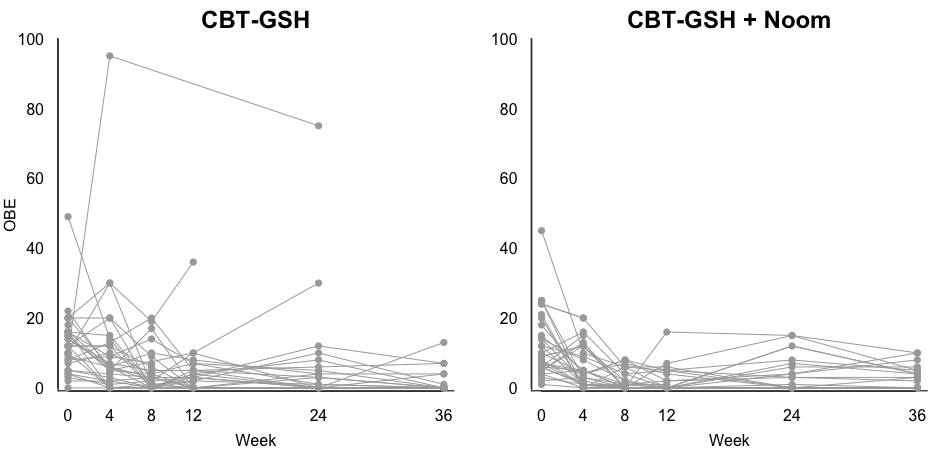
\includegraphics[width=\textwidth, height=\textheight, keepaspectratio]{Noom_paths.png}
   \end{center}
\caption{\emph{Fig.1 (a) and (b) show the OBE measurements for individuals in the CBT-GSH group and CBT-GSH + Noom group respectively. The horizontal axis shows the week and the vertical axis shows the instances of OBE. The gray dots represent OBE readings over time for each individual. }}
\end{figure}
%
Figure 2 displays the distribution of OBEs in each condition in each week.  We notice three characteristics of the data from these histograms.
\begin{enumerate}
\item{The distributions appear to condense around zero for both conditions over time} 
\item{The distributions in the CBT-GSH condition appear to have longer tails than those in the CBB-GSH+Noom condition}
\item{OBEs are count data; they must be nonnegative integers.}
\end{enumerate}
These three characteristics suggest that the appropriate model for OBEs is the Poisson distribution, because it is restricted to nonnegative integers and can concentrate its density around low numbers with a long tail.
%
\begin{figure}[H]
\begin{center}
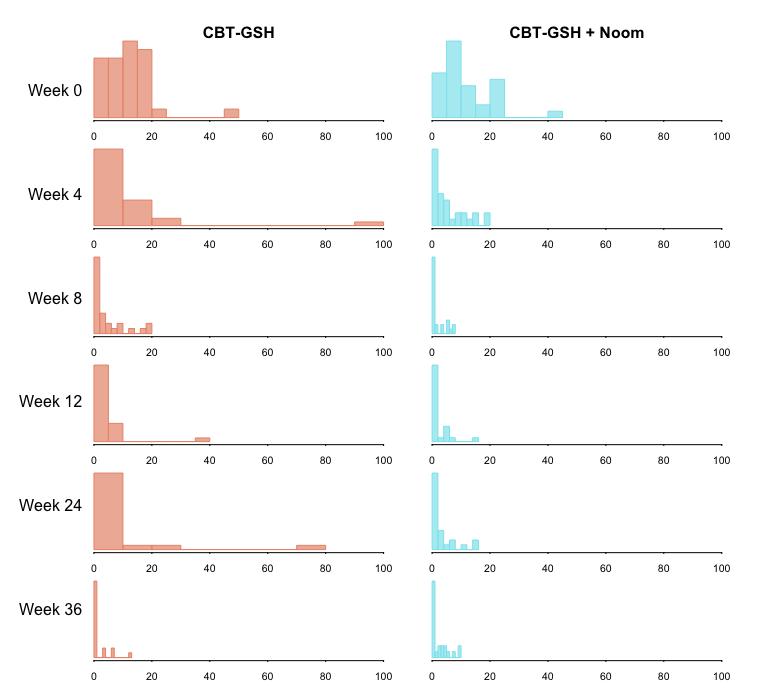
\includegraphics[width=\textwidth, height=\textheight, keepaspectratio]{noom_hist.png}
\end{center}
\caption{\emph{Histograms display the distribution of OBEs in each condition in each stage of the treatment. The orange and light blue histograms show the distribution of OBEs for the CBT-GSH and CBT-GSH  + Noom group respectively.}}
\end{figure}
%
\subsection*{Setting up a likelihood}

We analyze RCTs by modeling the outcome of interest (in this case OBE) as a function of the treatment and all available pre-treatment covariates.  The coefficients associated with the treatment reveal the average treatment effects.  Inclusion of all available pre-treatment covariates accounts for variation in the outcome variable, decreasing uncertainly around treatment effects and providing the model with more predictive power.  We conduct \emph{intent-to-treat} analysis, meaning that our inferences will be based on initial treatment assignment, and will not account for mid-experiment dropouts. \\
The outcome variable is restricted to be nonnegative integers, so we fit a Poisson regression model, with hierarchies on individuals, time periods, and treatment effects.  For each individual in each time period, the number of OBEs follows a Poisson distribution, with a mean dependent on the characteristics of the individual and the time period.  
\begin{align}
OBE_{i,t} &\sim Poisson(\lambda_{i,t}) \\
\lambda_{i,t} &= exp(\alpha_i + \beta_t + \gamma_tT_i + X_i\theta) \\
T_i &=
    \begin{cases}
      0, & \text{if}\ CBT-GSH \\
      1, & \text{if}\ CBT-GSH + Noom \\
    \end{cases}
\end{align}
$\alpha$ is an individual-specific intercept, $\beta$ is a time-specific intercept, $\gamma$ is a time-specific treatment effect, $T$ is a treatment indicator, $X$ is a matrix of individual level covariates (age, sex, race, etc), and $\theta$ is a vector of effects. Subscripts $i = 1, ..., 66$ indicate individuals and subscripts $t = 0, 4, 8, 12, 24, 36$ indicate time periods.

\subsection*{Choosing a prior distribution}
Table 1 has a list of different sources from which prior information has been obtained for this experiment. It aims to summarize the various methods which a researcher can use to incorporate prior information into the modeling process. There is a rich literature on binge-eating disorders and bulimia nervosa studies, implying a large amount of prior information. This makes analysis of similar RCTs amenable to Bayesian methods.
%
\begin{table}[H]
\centering
\begin{tabular}{r l}
  Source of Prior Information &  \\ 
  \hline  \vspace{0.25em}
  Experimental Design & Outcome variable is nonnegative integers \\
  \vspace{0.25em}
  Literature & Treatment effect size is small \\
                  & A large number of zeros in OBE data due to remission\\
  Exploratory Data Analysis & There is variation in OBEs at the individual level \\
					  & There is variation in OBEs over time \\
                                            & Treatment effects may vary over time \\
    \hline
\end{tabular}
\caption{\emph{Sources of prior information.}}
\end{table}
%
We believe that individual-level intercepts are simultaneously unique to the individual and common to the population; that is, each individual has their own baseline predilection to engage in eating disorder behavior, but their baseline predilections are not drastically different from each other.  We operationalize this concept by modeling all individual-level intercepts as coming from a common distribution, with \emph{hyperparameters} $\mu_{\alpha}$ and $\tau_{\alpha}$.
%
\begin{align}
\alpha_i \sim Normal(\mu_{\alpha}, \tau_{\alpha}) \ \forall \ i \in 1,...,66
\end{align} 
%
Similarly, we believe that time-specific treatment effects may be unique to each period but similar over time. We operationalize this concept by modeling all time-specific treatment effects $\gamma$ as coming from a common distribution, with \emph{hyperparameters} $\mu_{\gamma}$ and $\tau_{\gamma}$.
%
\begin{align}
\gamma_t \sim Normal(\mu_{\gamma}, \tau_{\gamma}) \ \forall \ t \in 0, 4, 8, 12, 24, 36
\end{align} 
%
$\mu_{\gamma}$ is the \emph{grand mean}, the overall treatment effect; $\tau_{\gamma}$ is the variation in treatment effects over time; and each individual $\gamma_t$ is a time-period specific treatment effect.  This approach has a natural smoothing effect: any extreme estimates of $\gamma_t$ will be partially-pooled back toward the grand mean $\mu_{\gamma}$.\\
%
We assign the following prior and hyperprior distributions:
\begin{align}
\mu_{\alpha} &\sim Normal(5, 5) \\
\tau_{\alpha} &\sim Cauchy^+(0, 30) \\
\mu_{\gamma} &\sim Normal(0, 5) \\
\tau_{\gamma} &\sim Cauchy^+(0, 30) \\
\theta &\sim Normal(0, 1)
\end{align}
%
The normal distributions around the individual and treatment effects allow us to guide the model to the appropriate range of parameter values, but with wide enough variance (5 in each case) to let the model find its own way in that range.  Half cauchy priors on the variance parameters are weakly informative, with much of their mass around zero but gentle slopes in their tails, which have been shown to be effective prior distributions for variance parameters [Gelman, 2006].

\subsection{Model estimation and results}
We estimate this model with \emph{Hamilton Monte-Carlo} in Stan.  Model code is appended to this document.  We find that the model converges with four chains of 2000 iterations each (see Table 2).
Model results are displayed in Table 2.  Results suggest that using the Noom Monitor smartphone application during CBT-GSH may slightly decrease OBEs.  There is evidence that the treatment effect varies over time, with the Noom effect being slightly more pronounced during stages 4, 8, 12 and 24 of therapy but decreasing by week 36.\\

\begin{table}[H]
\centering
\begin{tabular}{r c c c c c}
  \hline
 & mean & 25\% & 50\% & 75\% & R-hat\\ 
  \hline
  $\gamma_0$ & 0.18 & -0.45 & 0.15 & 0.78 & 1   \\ 
  $\gamma_4$ & -0.43 & -1.05 & -0.46 & 0.16 & 1   \\ 
  $\gamma_8$ & -0.70 & -1.33 & -0.71 & -0.10   & 1\\  
  $\gamma_{12}$ & -0.65 & -1.28 & -0.68 & -0.04   & 1\\  
  $\gamma_{24}$ & -0.72 & -1.34 & -0.75 & -0.11  & 1\\  
  $\gamma_{36}$ & 0.21 & -0.42 & 0.19 & 0.82 & 1 \\ 
  \hline \hline
  $\mu_{\gamma}$ & -0.34 & -0.98 & -0.36 & 0.26  & 1\\ 
  $\tau_{\gamma}$ & 0.64 & 0.43 & 0.56 & 0.77  & 1\\ 
   \hline
\end{tabular}
\caption{\emph{Table displays model results for Noom effects in all six time periods and grand mean and variance parameters.}}
\end{table}


\subsection{Model checking, comparison, and expansion}
Before using our model to make inferences about time-specific treatment effects, we check its fit by comparing model-simulated OBE to data OBE.  If model simulations do not track the data well, we may want to revisit our model's assumptions before trusting its inferences.  If the model's simulations recover patterns in the data, we are more inclined to trust its inferences. \\
Figure 3 displays OBEs in each period for each individual in each treatment group, from raw data (upper plots) and model simulations (lowers plots).  Black lines display means for each period.  This suggests that the model is able to pick up on the key variables that determine OBE over time for the duration of this experiment.
%
\begin{figure}[H]
\begin{center}
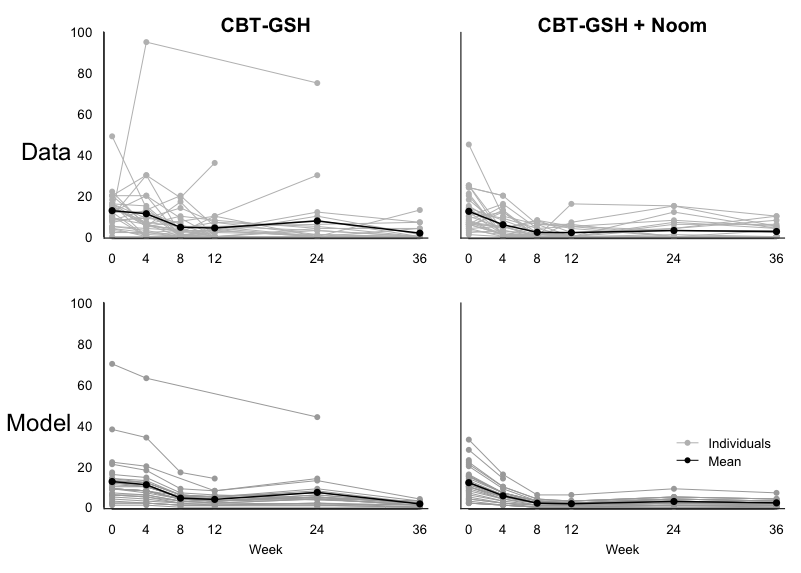
\includegraphics[width=\textwidth, height=\textheight, keepaspectratio]{ppc_sims.png}
\caption{\emph{Fig.3 (a) and (b) in the upper row show OBEs in each period for each individual in CBT - GSH and CBT-GSH + Noom respectively. Black dots represent mean estimate for each  period. Fig.3 (c) and (d) in the lower row show the simulated OBEs for each individual in CBT - GSH and CBT-GSH + Noom respectively. Black dots represent means from the simulated data for each period. The horizontal axis shows the week and the vertical axis shows the instances of OBE.}}
\end{center}
\end{figure}
%
Another way to check the fit of the model is by comparing simulated data directly against the raw data.  Figure 4 shows this for both treatment conditions.  Simulated data for the Noom condition appears to better track the raw data than simulated data for the no Noom condition.  This is unsurprising, since the no Noom condition tended to have more outliers, which we would not expect (or want) our model to pick up perfectly from such a small sample.  
%
\begin{figure}[H]
\begin{center}
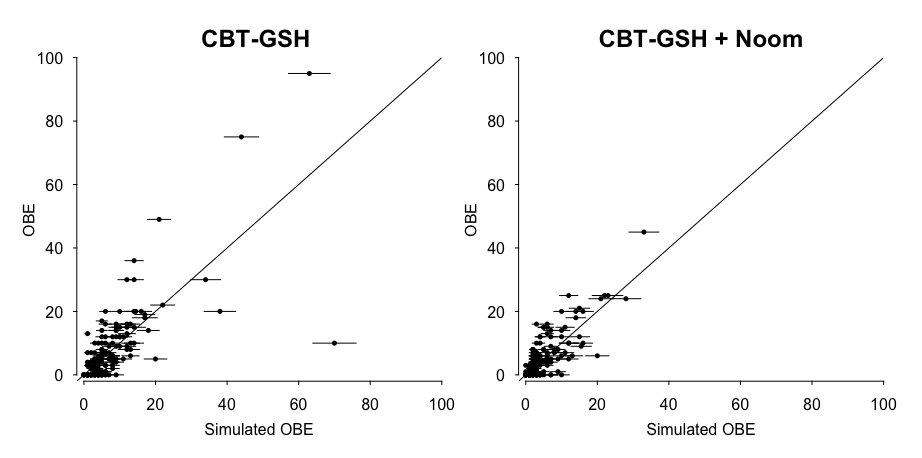
\includegraphics[width=\textwidth, height=\textheight, keepaspectratio]{obe_ppcs.png}
\caption{\emph{Fig. 4(a) and (b) show the predicted OBE vs. the actual OBE data for CBT - GSH and CBT- GSH + Noom respectively. The horizontal axis shows the simulated OBE and the vertical axis shows the actual OBE. The black dots are the points that represent this and the lines around them show 50\% intervals around the predictions. The upward sloping line is the 45 degree line.}}
\end{center}
\end{figure}
%
We conclude our model evaluations by mapping modeled density curves for each condition in each time period over the histograms in Figure 2.  Figure 5 shows that our model is able to broadly pick up on the patterns in the data over time and between treatment conditions. We see that the density curves clearly peak at lower values close to zero and have long tails, correctly capturing the pattern in the OBE data.

\begin{figure}[H]
\centering
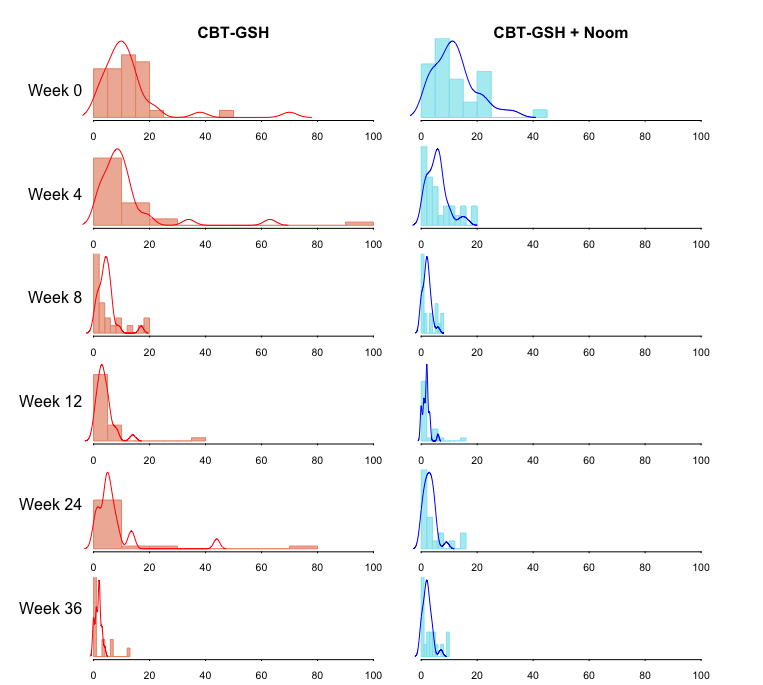
\includegraphics[width=\textwidth, height=\textheight, keepaspectratio]{ppc_hist_dens.png}
\caption{\emph{Histograms display the distribution of OBEs in each condition in each stage of the treatment. The orange and light blue histograms show the distribution of OBEs for the CBT-GSH and CBT-GSH  + Noom group respectively. The red and blue lines show the predicted density curves obtained from the simulations.}}
\end{figure}
Figure 6 displays the simulated OBE for both treatment groups (upper plot) and smoothed treatment effects (lower plot).  In each measurement period, simulated OBE are higher for the CBT - GSH condition than for the CBT - GSH + Noom condition, with some of the difference likely attributable to use of the Noom Monitor smartphone app.  This shows that the app has an effect on lowering episodes of binge eating.

\begin{figure}[H]
\begin{center}
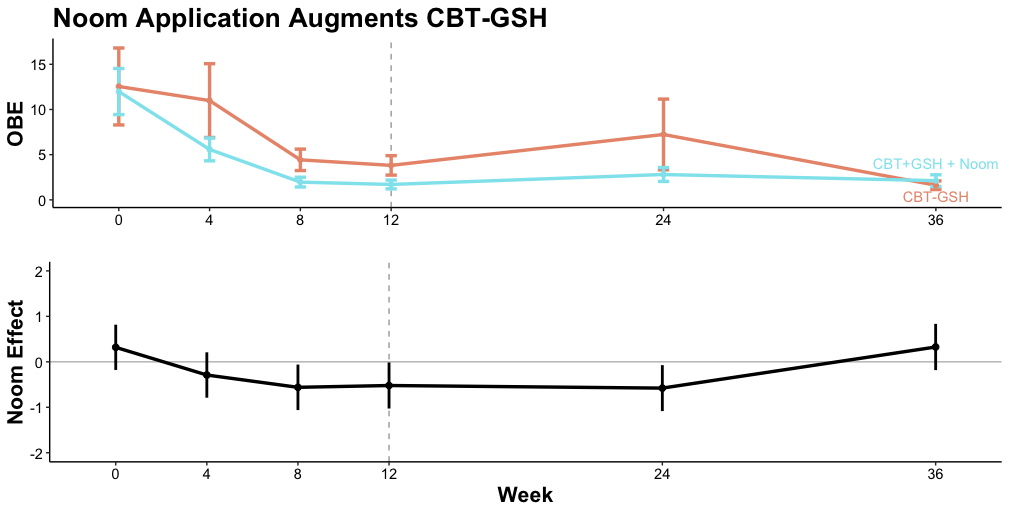
\includegraphics[width=\textwidth, height=\textheight, keepaspectratio]{noom_effect.png}
\caption{\emph{Fig. 6(a) the upper plot shows the simulated OBE in each time period. The CBT - GSH condition is in orange and the CBT - GSH + Noom condition is in orange. The bars around each point show the 95\% interval. Fig. 6(b) the lower plot shows the treatment effect for each period with the bars showing the 50\% interval. The horizontal axis shows the time period and the vertical axis for Fig.6 (a) shows the instances of OBE and for Fig.6 (b) shows the treatment effect of the Noom app.}}
\end{center}
\end{figure}


\section{Conclusion}

\newpage
\section{Appendix}
\begin{sexylisting}{Stan code}
data{
  int N;
  int N_time;
  int N_ppl;
  int OBE[N];
  vector[N] tmt;
  int person_id[N];
  int time_id[N];
  int sex[N];
  int age[N];
  int black[N];
  int other_race[N];
  int hisp[N];
  int bn[N];
}
parameters{
  real alpha[N_ppl];
  real mu_alpha;
  real<lower = 0> tau_alpha;
  real alpha_sex;
  real alpha_age;
  real alpha_black;
  real alpha_other;
  real alpha_hisp;
  real alpha_bn;
  real beta[N_time];
  real gamma[N_time];
  real mu_gamma;
  real<lower = 0> tau_gamma;
}
\end{sexylisting}
\begin{sexylisting}{Stan code contd.}
model{
  for(i in 1:N) {
    OBE[i] ~ poisson_log(alpha[person_id[i]] + alpha_sex*sex[i] 
                         + alpha_black*black[i] 
                         + alpha_other*other_race[i]
                         + alpha_hisp*hisp[i] + alpha_bn*bn[i]
                         + beta[time_id[i]] + alpha_age*age[i]
                         + gamma[time_id[i]]*tmt[i]);
  }
  alpha ~ normal(mu_alpha, tau_alpha);
  mu_alpha ~ normal(5, 2);
  tau_alpha ~ cauchy(0, 50);
  alpha_black ~ normal(0, 1);
  alpha_sex ~ normal(0, 1);
  alpha_other ~ normal(0, 1);
  alpha_hisp ~ normal(0, 1);
  alpha_bn ~ normal(0, 1);
  gamma ~ normal(mu_gamma, tau_gamma);
  mu_gamma ~ normal(0, 2);
  tau_gamma ~ cauchy(0, 30);
}
\end{sexylisting}
\begin{sexylisting}{Stan code contd.}
generated quantities{
  real OBE_pred[N];
  for(i in 1:N) {
    OBE_pred[i] = poisson_log_rng(alpha[person_id[i]] 
                                  + alpha_sex*sex[i] 
                                  + alpha_black*black[i] 
                                  + alpha_other*other_race[i]
                                  + alpha_hisp*hisp[i] 
                                  + alpha_bn*bn[i]
                                  + beta[time_id[i]] 
                                  + alpha_age*age[i]
                                  + gamma[time_id[i]]*tmt[i]);
  }
}
\end{sexylisting}

\begin{thebibliography}{9}

\bibitem{A Conceptual Introduction to Hamiltonian Monte Carlo}
Betancourt M (2017).
\textit{``A Conceptual Introduction to Hamiltonian Monte Carlo"} 
arXiv:1701.02434 [stat.ME]

\bibitem{Bayesian Data Analysis}
Gelman A, Carlin J.B, Stern H.S, Rubin D.B (2013).
\textit{``Bayesian Data Analysis"}
ISBN 0-412-03991-5, Chapman and Hall, New York

\bibitem{Prior distributions for variance parameters in hierarchical models(Comment on Article by Browne and Draper)}
Gelman A (2006).
\textit{``Prior distributions for variance parameters in hierarchical models(Comment on Article by Browne and Draper)"}
2006, International Society for Bayesian Analysis, Number 3, pp. 515 - 534.

\bibitem{Data Analysis Using Regression and Multilevel/Hierarchical Models}
Gelman A, Hill J (2007).
\textit{``Data Analysis Using Regression and Multilevel/Hierarchical Models"}
ISBN-13 978-0-521-68689-1, Published in the United States of America by Cambridge University Press, New York

\bibitem{Benefits and limitations of randomized controlled trials}
Gelman A (2017).
\textit{``Data Analysis Using Regression and Multilevel/Hierarchical Models"}
http://www.stat.columbia.edu/~gelman/research/published/causal_ssm.pdf

\bibitem{The benefits of using semi-continuous and continuous models to analyze binge eating data: A Monte Carlo investigation}
Grotzinger, A, Hildebrandt, T, and Yu, J. (2015). 
\textit{``The benefits of using semi-continuous and continuous models to analyze binge eating data: A Monte Carlo investigation."}
 Int J Eat Disord, 48(6), 746-758. doi:10.1002/eat.22351.
 
 \bibitem{Randomized controlled trial comparing smartphone assisted
versus traditional guided self-help for adults with binge eating}
Hildebrandt T, Michaelides A, Mackinnon D, Greif R, DeBar L, Sysko R (2017)
\textit{``Randomized controlled trial comparing smartphone assisted
versus traditional guided self-help for adults with binge eating"}
Int J Eat Disord. 2017 Nov;50(11):1313-1322. doi: 10.1002/eat.22781.

\bibitem{Stan}
Stan Development Team. 2016. 
\textit{RStan: the R interface to Stan}, Version 2.10.1.   
\texttt{http://mc-stan.org}

\bibitem{Stan}
Stan Development Team.
\textit{``Prior Choice Recommendations"}
\texttt{https://github.com/stan-dev/stan/wiki/Prior-Choice-Recommendations}

\end{thebibliography}



\end{document}